\documentclass[12pt, a4]{article}
\usepackage[english]{babel}
\usepackage[utf8]{inputenc}
\usepackage{fullpage}
\usepackage{listings}
\usepackage{graphicx}
\usepackage{color}

%Syntax highlighting
\definecolor{blue-violet}{rgb}{0.54, 0.17, 0.89}
\definecolor{ao}{rgb}{0.0, 0.5, 0.0}
\definecolor{amaranth}{rgb}{0.9, 0.17, 0.31}
\definecolor{ballblue}{rgb}{0.13, 0.67, 0.8}
\definecolor{onyx}{rgb}{0.06, 0.06, 0.06}


\lstset{
  breaklines=true,                 % automatic line breaking only at whitespace
  captionpos=b,                    % sets the caption-position to bottom
  breakatwhitespace=false,
  keepspaces=true,
  numbers=left,
  numbersep=5pt,
  showspaces=false,
  showstringspaces=false,
  showtabs=false,
  tabsize=4,  
  backgroundcolor=\color{white},   % choose the background color
  commentstyle=\color{ao},    % comment style
  keywordstyle=\color{amaranth},    % keyword style
  stringstyle=\color{blue-violet},    % string literal style
  numberstyle=\tiny\color{ballblue},	   % number style
  basicstyle=\ttfamily\footnotesize\color{onyx} % size of fonts used for the code
}


%Document Header
\title{\textbf{Department of CSE\\SSN College of Engineering}}
\author{\textbf{Vishakan Subramanian - 18 5001 196 - Semester VI}}
\date{09 March 2021}

\begin{document}
\maketitle
\hrule
\section*{\center{UCS 1611 - Internet Programming Lab}}
\hrule
\bigskip

%Assignment Details
\subsection*{\center{\textbf{Exercise 3: JavaScript Event Handling Mechanisms, DOM}}}
\subsection*{\flushleft{Learning Objective:}}
\begin{flushleft}
Generate a registration form for a hospital to register new patient details as
below:

\begin{enumerate}
\item Assign a title for the registration form(TextView- textSize, textStyle ,
typeface)
\item Name. Specify some font and colour. (text, onfocus, onblur, oninvalid)
\item Address (textarea, onselect)
\item Age (onkeypress)
\item Date of Birth (date)
\item Gender (RadioButton)
\item Marital Status (select, onchange)
\item Contact Number (oninvalid)
\item Addiction (text area, use drag and drop from a list-select)
\item Display a digital clock on the top right corner of the webpage
\item Submit (Button, onclick create a new page and display the contents in table format)
\item Reset (Button, onclick)
\end{enumerate}

Write a JS program to develop a memory matching game.

\begin{enumerate}
\item Display a timer, Score card.
\item Arrange even number of pairs. (Minimum 5)
\item Shuffle the cards, face down, in rows.
\item Score card changes whenever a pair is found.
\item On click a card, it should flip (event handling).
\item When a match is found, remove the cards using DOM.
\item Set 3 levels.
\item When the player moves to next level, set a new timer with less time
duration.
\item Mandatory concepts – Event handling, DOM.
\end{enumerate}
 
\end{flushleft}

%Code
\newpage
\subsection*{\flushleft{Code - Registration Page HTML:}}
\begin{flushleft}
\lstinputlisting[language = HTML]{index.html}
\end{flushleft}

\newpage
\subsection*{\flushleft{Code - Submission Page HTML:}}
\begin{flushleft}
\lstinputlisting[language = HTML]{submission.html}
\end{flushleft}

\newpage
\subsection*{\flushleft{Code - Registration Page JS:}}
\begin{flushleft}
\lstinputlisting[]{js/index.js}
\end{flushleft}

\newpage
\subsection*{\flushleft{Code - Submission Page JS:}}
\begin{flushleft}
\lstinputlisting[]{js/submission.js}
\end{flushleft}

\newpage
\subsection*{\flushleft{Code - Registration and Submission Page CSS:}}
\begin{flushleft}
\lstinputlisting[]{css/styles.css}
\end{flushleft}

\newpage
\subsection*{\flushleft{Code - Game Page HTML:}}
\begin{flushleft}
\lstinputlisting[language = HTML]{game.html}
\end{flushleft}

\newpage
\subsection*{\flushleft{Code - Game Page JS:}}
\begin{flushleft}
\lstinputlisting[]{js/gamescript.js}
\end{flushleft}

\newpage
\subsection*{\flushleft{Code - Game Page CSS:}}
\begin{flushleft}
\lstinputlisting[]{css/gamestyles.css}
\end{flushleft}

%Output
\newpage
\subsection*{\flushleft{Output - Registration Page:}}
\begin{figure}[h]
\centering
\caption{Browser Output: Registration Page.}
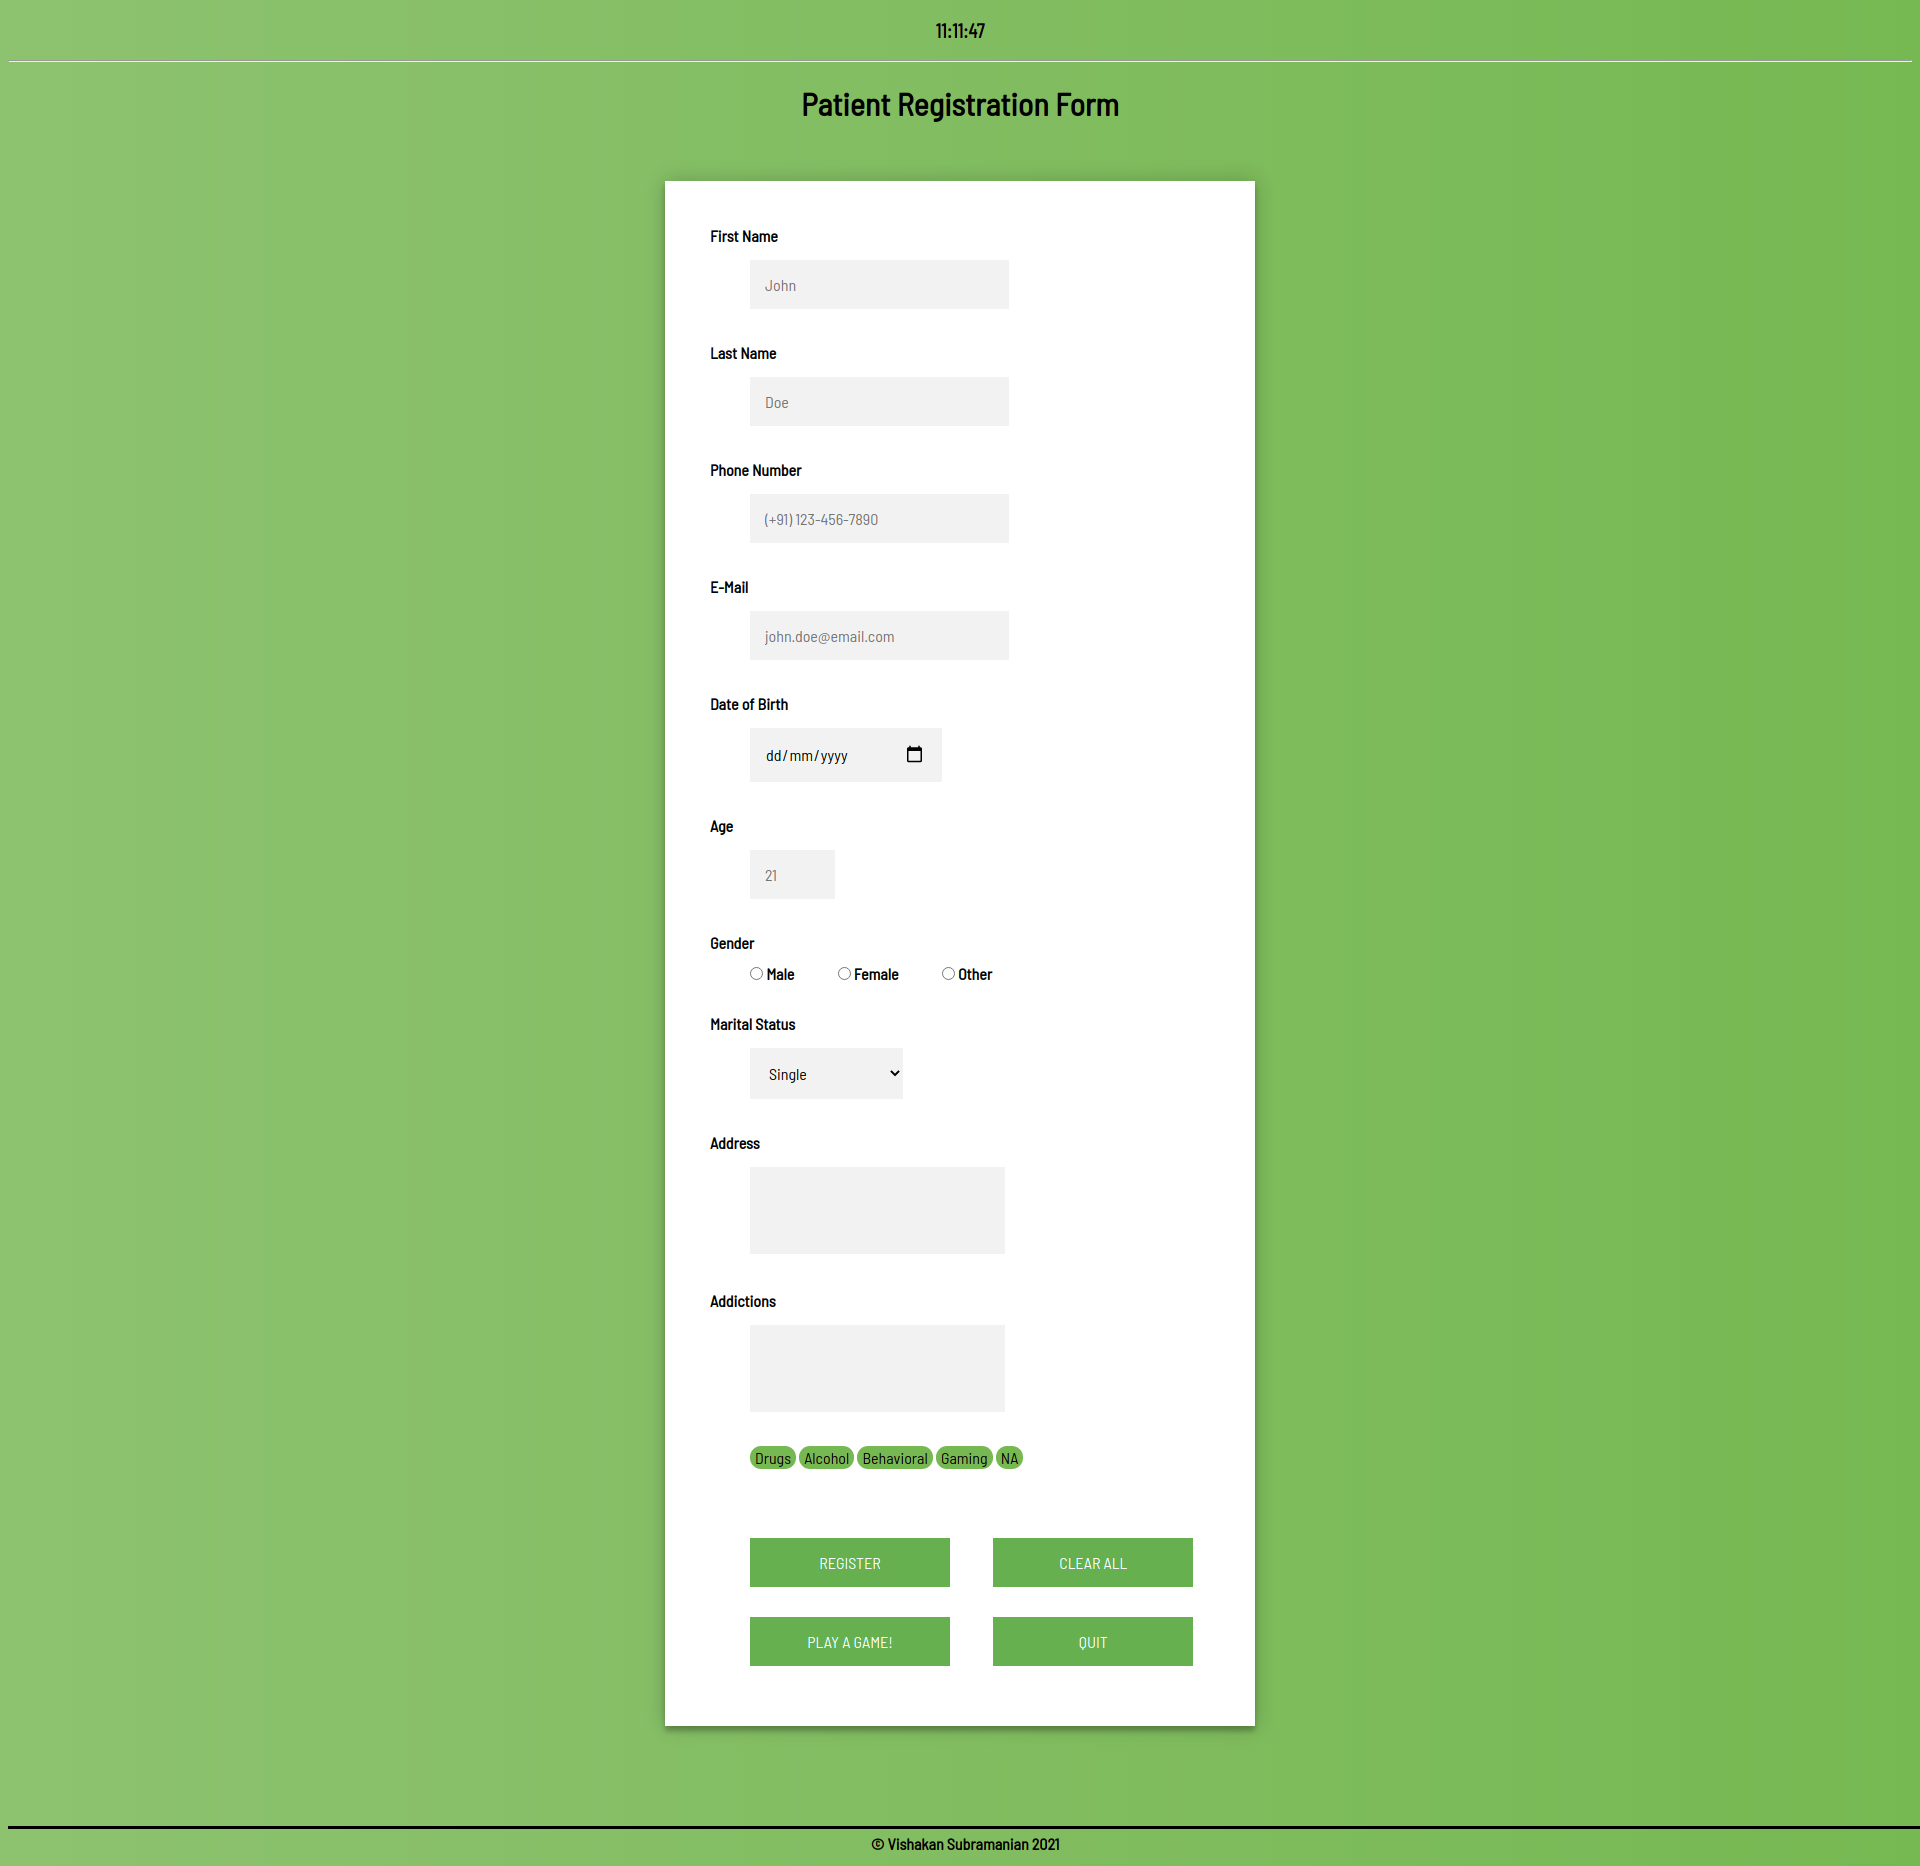
\includegraphics[height=15cm, width=18cm]{Output/RegForm.png}
\end{figure}

\newpage
\subsection*{\flushleft{Output - Registration Page Filled:}}
\begin{figure}[h]
\centering
\caption{Browser Output: Registration Page Filled.}
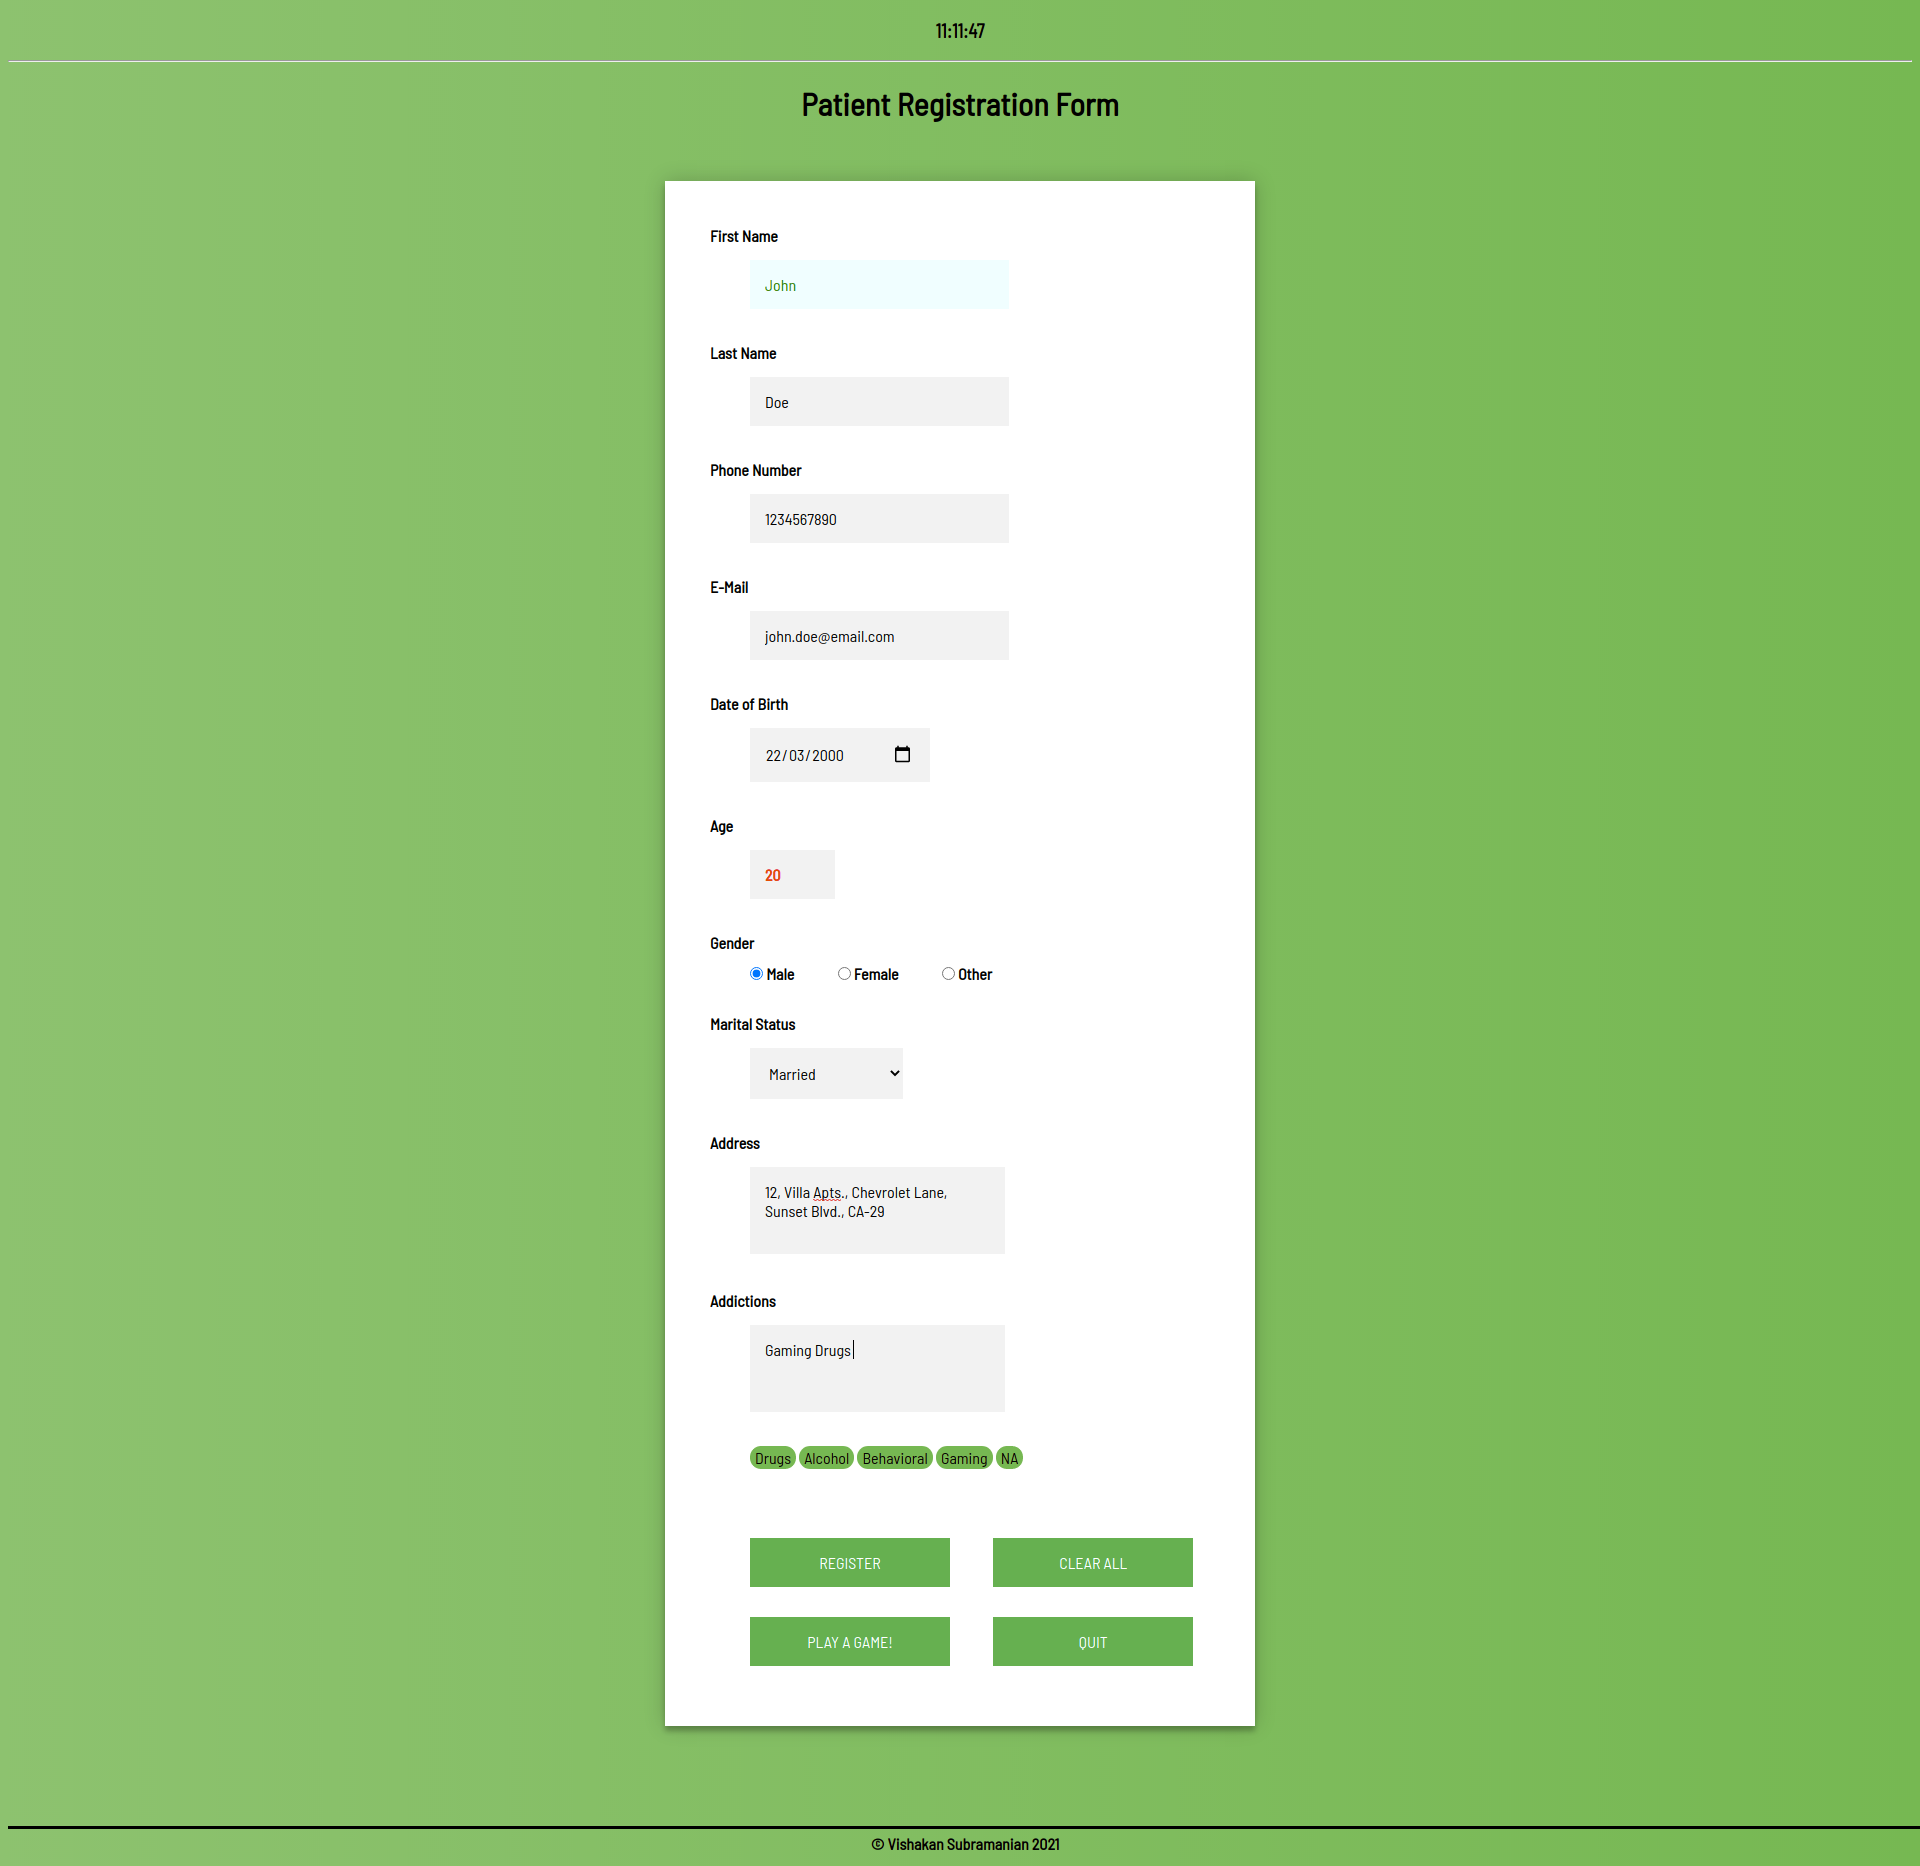
\includegraphics[height=15cm, width=18cm]{Output/RegFormFilled.png}
\end{figure}

\newpage
\subsection*{\flushleft{Output - Submission Page:}}
\begin{figure}[h]
\centering
\caption{Browser Output: Submission Page.}
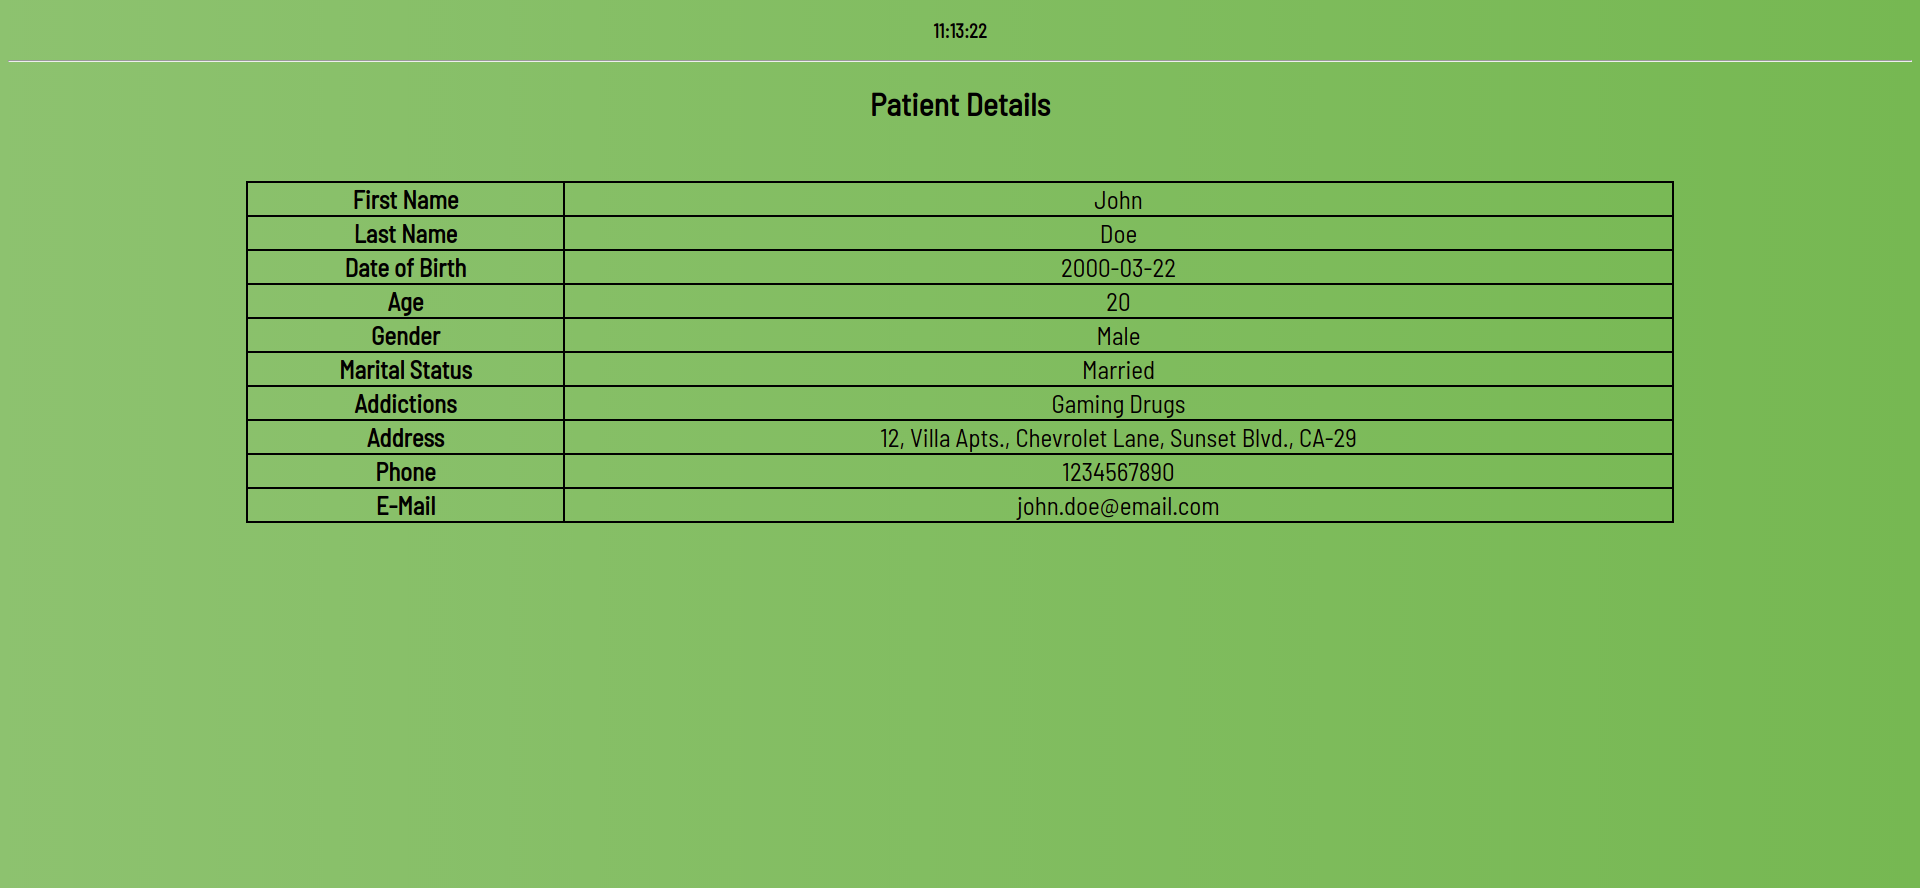
\includegraphics[height=15cm, width=18cm]{Output/FormTable.png}
\end{figure}

\newpage
\subsection*{\flushleft{Output - Game Page:}}
\begin{figure}[h]
\centering
\caption{Browser Output: Game Page.}
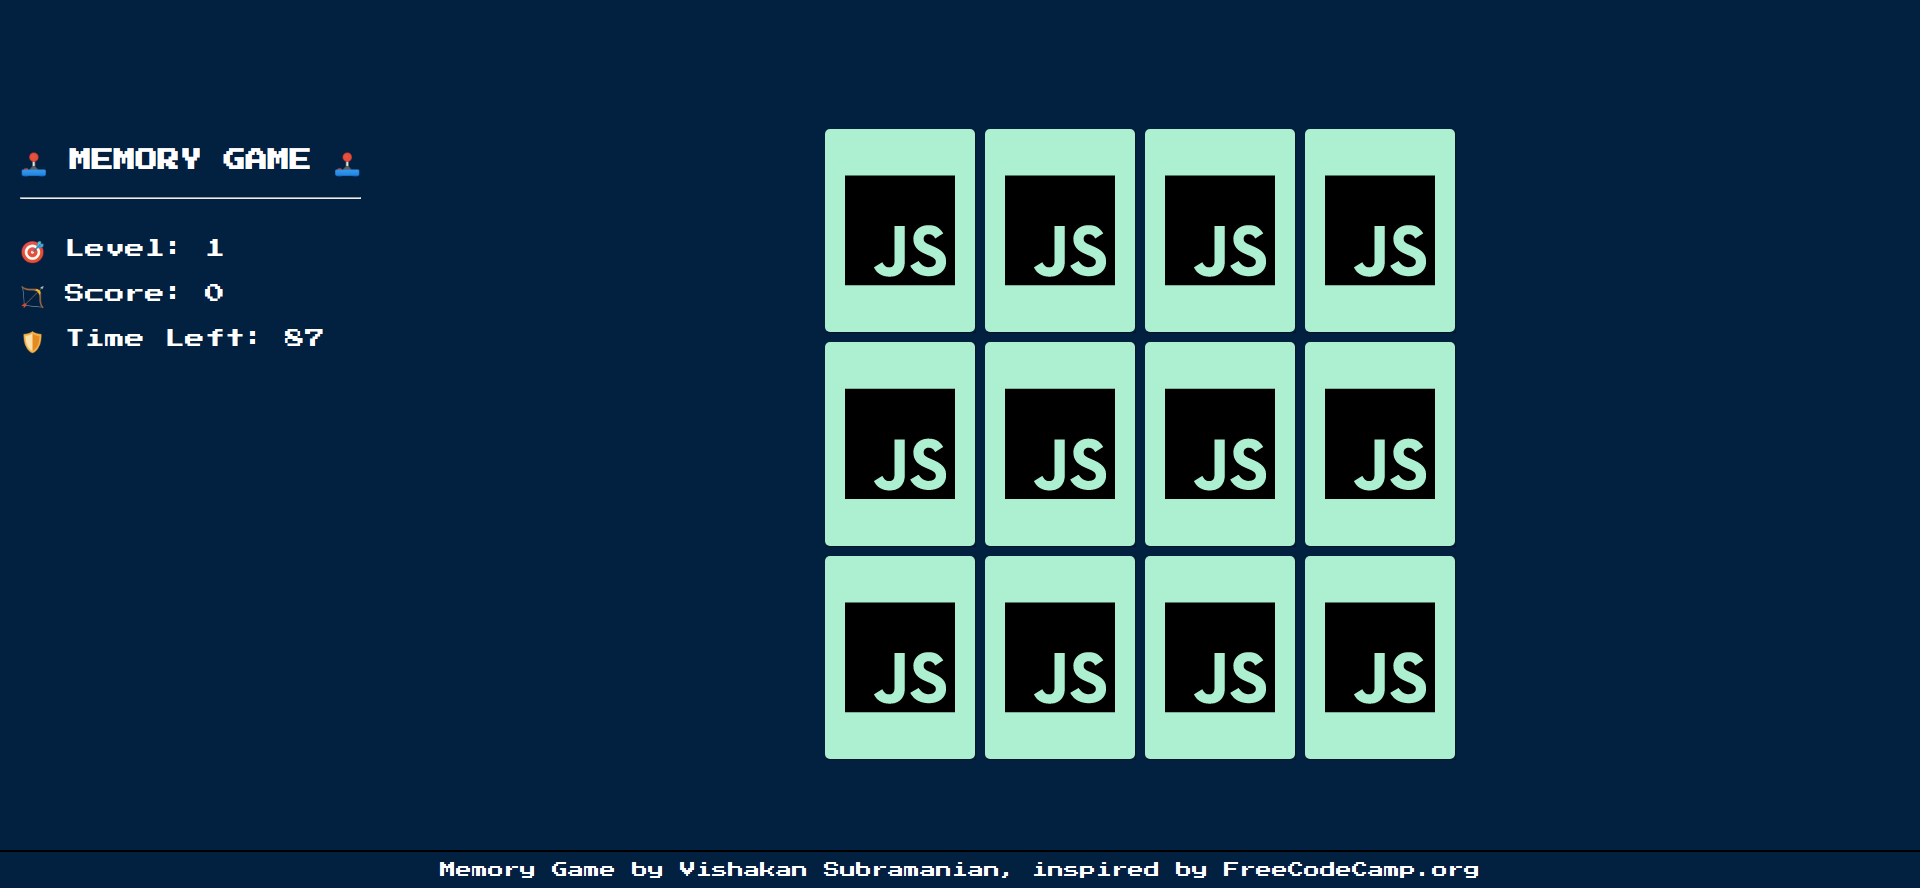
\includegraphics[height=15cm, width=18cm]{Output/MemGame.png}
\end{figure}

\newpage
\subsection*{\flushleft{Output - Game Finished:}}
\begin{figure}[h]
\centering
\caption{Browser Output: Game Finished Page.}
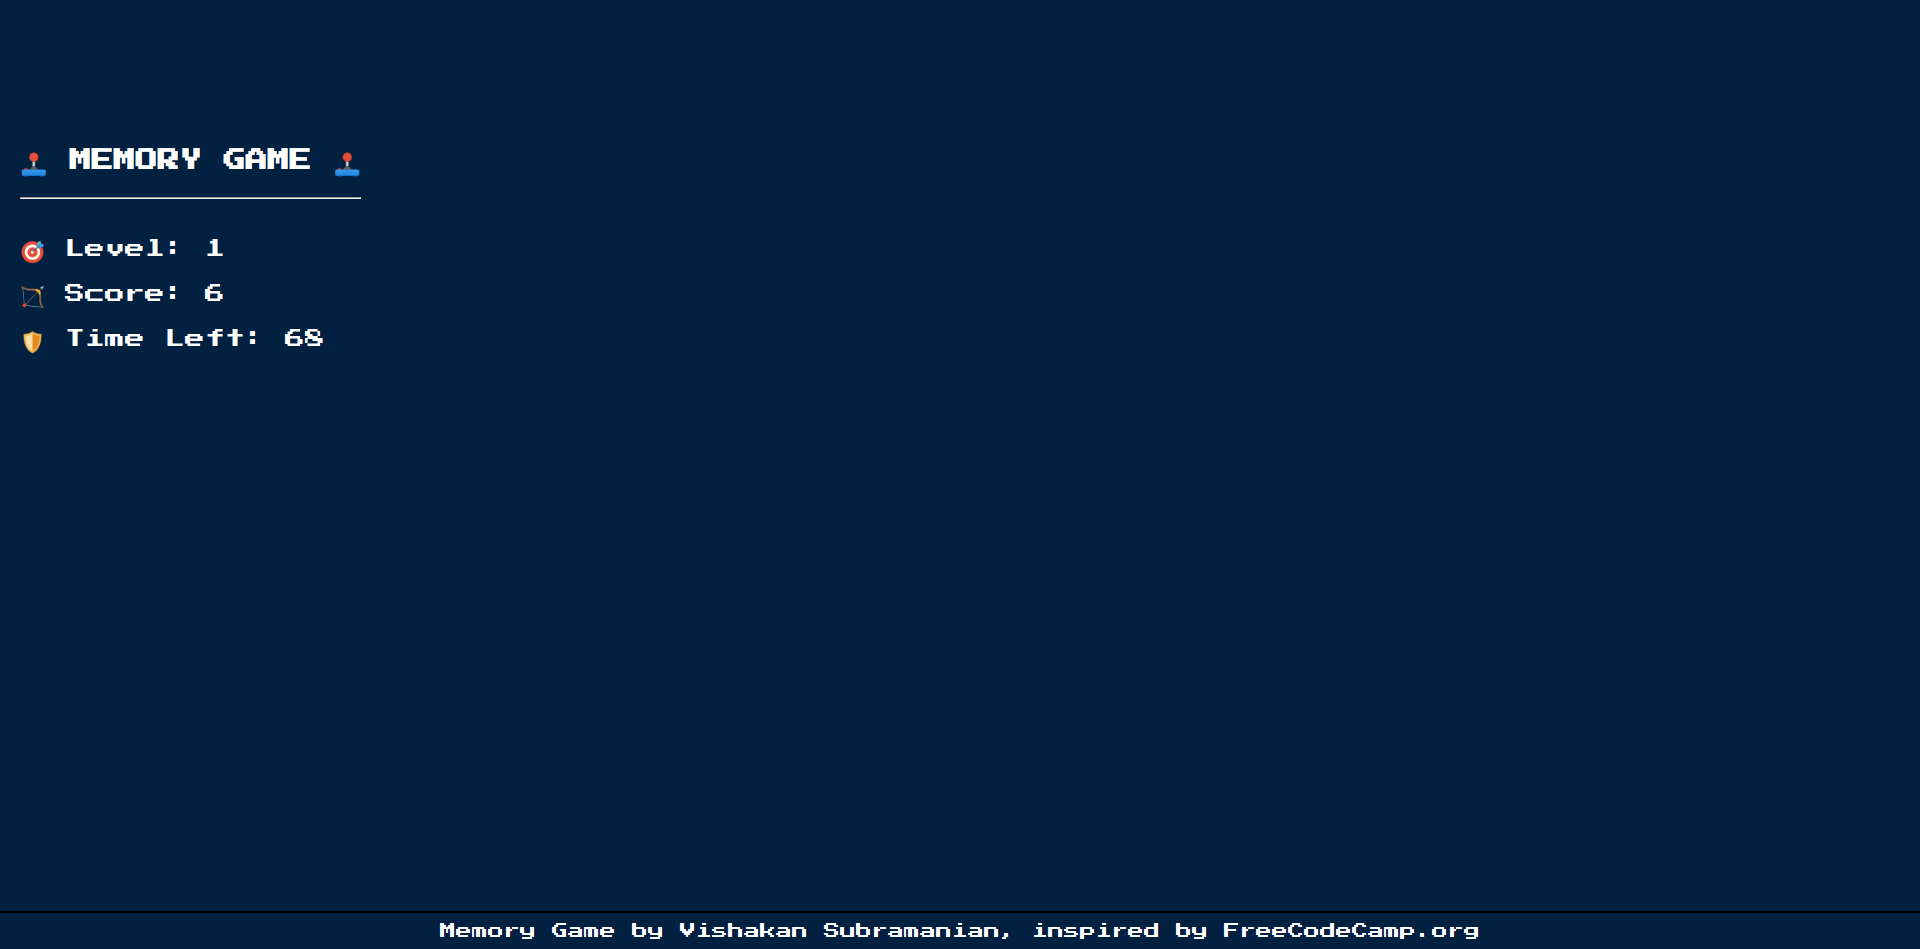
\includegraphics[height=15cm, width=18cm]{Output/GameFin.png}
\end{figure}

\newpage
\subsection*{\flushleft{Output - Game Page (Level 2):}}
\begin{figure}[h]
\centering
\caption{Browser Output: Game Page (Level 2).}
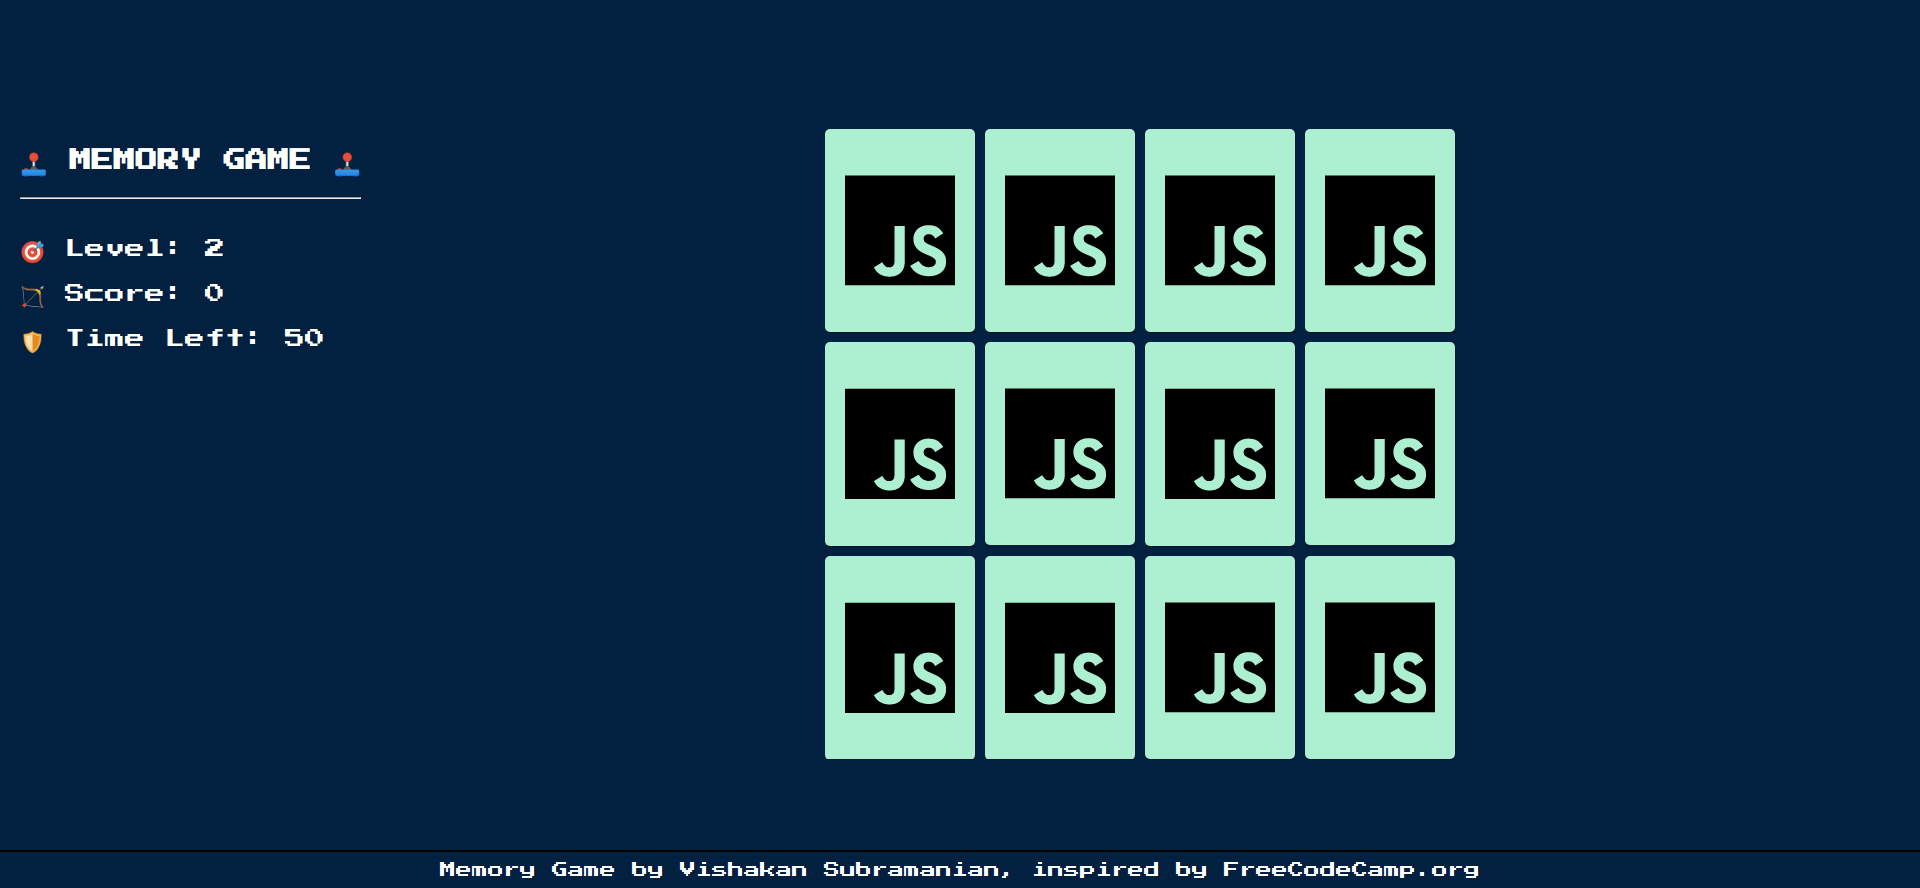
\includegraphics[height=15cm, width=18cm]{Output/NextLevel.png}
\end{figure}


%Learning Outcome
\newpage
\subsection*{\flushleft{Learning Outcome:}}
\begin{itemize}

\item From the experiment, I learnt to implement a detailed form.
\item I learnt about basic JavaScript syntax.
\item I learnt basic DOM manipulation with methods such as getElementById(), querySelectorAll(), etc.
\item I was able to implement a simple drag-and-drop element using JavaScript.
\item I learnt how to deliver form data to another webpage using the POST method and URLSearchParams object.
\item I was able to implement actions for different events like onfocus, onblur, oninvalid etc.
\item I implemented a simple memory game using JavaScript.
\item I learnt to implement timers in JavaScript.
\item I understood about removeEventListener() and addEventListener() methods.
\item I was able to implement level hierarchy in the game using JavaScript.
\item I learnt how to add a class to an HTML element through JavaScript using classList.
\item I learnt how to shuffle elements in the HTML page using the CSS order property and Math.random() in JavaScript.
\item I learnt how to implement user-defined functions in JavaScript.
\item I was able to manipulate the values of HTML content like the game's score and time remaining using JavaScript.

\end{itemize}

\end{document}
